\documentclass[format=sigconf]{acmart}
\usepackage[english]{babel}
\usepackage{float}
\usepackage[labelfont=bf,textfont=md]{caption}
\usepackage{graphicx}
\usepackage{xcolor}
\usepackage{minted}
\usepackage{hyperref}
\usepackage[all]{hypcap}
\usemintedstyle[glsl]{default}
\usemintedstyle[common-lisp]{default}
\newmintinline[code]{text}{}
\bibliographystyle{unsrt}

\hypersetup{
  colorlinks,
  linkcolor={red!50!black},
  citecolor={blue!50!black},
  urlcolor={blue!80!black}
}

\setcopyright{rightsretained}
\acmDOI{}
\acmISBN{978-2-9557474-2-1}
\acmConference[ELS'18]{the 11th European Lisp Symposium}{April 16--17 2018}{%
  Marbella, Spain}

\begin{document}

\title{Object Oriented Shader Composition Using CLOS}

\author{Nicolas Hafner}
\affiliation{%
  \institution{Shirakumo.org}
  \city{Zürich}
  \country{Switzerland}
}
\email{shinmera@tymoon.eu}

\begin{abstract}
  We present a new approach to applying object oriented principles to GPU programming via GLSL shaders. Using the CLOS Meta Object Protocol, shader code can be attached to classes within standard Lisp code and is automatically combined by the system according to inheritance rules. This approach results in a native coupling of both CPU and GPU logic, while preserving the advantages of object oriented inheritance and behaviour. The system allows the use of arbitrary shaders written directly in GLSL, without the need for language extensions.
\end{abstract}

\begin{CCSXML}
  <ccs2012>
  <concept>
  <concept_id>10011007.10010940.10010971.10010972.10010979</concept_id>
  <concept_desc>Software and its engineering~Object oriented architectures</concept_desc>
  <concept_significance>500</concept_significance>
  </concept>
  <concept>
  <concept_id>10011007.10010940.10010971.10011682</concept_id>
  <concept_desc>Software and its engineering~Abstraction, modeling and modularity</concept_desc>
  <concept_significance>500</concept_significance>
  </concept>
  <concept>
  <concept_id>10011007.10011006.10011066.10011067</concept_id>
  <concept_desc>Software and its engineering~Object oriented frameworks</concept_desc>
  <concept_significance>300</concept_significance>
  </concept>
  <concept>
  <concept_id>10011007.10011006.10011041.10011688</concept_id>
  <concept_desc>Software and its engineering~Parsers</concept_desc>
  <concept_significance>100</concept_significance>
  </concept>
  <concept>
  <concept_id>10010147.10010371</concept_id>
  <concept_desc>Computing methodologies~Computer graphics</concept_desc>
  <concept_significance>300</concept_significance>
  </concept>
  </ccs2012>
\end{CCSXML}

\ccsdesc[500]{Software and its engineering~Object oriented architectures}
\ccsdesc[300]{Software and its engineering~Abstraction, modeling and modularity}
\ccsdesc[300]{Software and its engineering~Object oriented frameworks}
\ccsdesc[100]{Software and its engineering~Parsers}
\ccsdesc[300]{Computing methodologies~Computer graphics}

\keywords{Common Lisp, GLSL, OpenGL, GPU, CLOS, MOP, Object Orientation}

\maketitle

\newpage

\def\abovecaptionskip{1pt}
\def\listingautorefname{listing}
\def\figureautorefname{figure}

\section{Introduction}\label{section:1}
In modern real-time computer graphics applications, advanced effects and GPU computations require the use of a programmable graphics pipeline. This is usually done using domain-specific languages. The programmer passes the programs as textual source code to the graphics driver, which then compiles it down to GPU instructions.\\

For OpenGL, this language is called GLSL\cite{rost2009opengl} and follows a mostly C-like syntax. A program written in GLSL is called a shader and is used to fill one of several stages in the graphics pipeline. Whenever a primitive is rendered, these shaders are executed on the GPU, each providing a particular stage of processing until finally an image is produced. \\

However, only a single shader can live in a particular stage at a time. This limitation presents an issue for modularity, as effects represented by shaders cannot be easily combined. Instead, it is usually the task of a programmer to craft a single shader for each stage that produces the desired results. \\

In this paper we present a new solution to this problem that is accomplished in two steps. The first step is the parsing and manipulation of native GLSL code. The second step is the integration of shader code into the Common Lisp Object System to allow for automatic combination through inheritance.

\section{Related Work}\label{section:2}
Several different approaches to shader combination exist today. \\

Trapp et al\cite{trapp2007automated} use additional constructs introduced to GLSL and a preprocessor to combine effects. Their approach differs from ours in that we do not extend GLSL syntax in any way and do not present a standard interface to use between shader fragments. \\

McCool et al.\cite{mccool2002shader} present an extension of the C++ language to allow writing GLSL-like code in C++ source. Shader fragments are parsed into an abstract syntax that can be used to perform static analysis and combination of fragments. Combination is however not automatic and needs to be explicitly requested by the programmer. \\

Kuck\cite{kuck2007object} presents an evolution of McCool's approach by allowing the use of C++ method declarations for shader function definitions. In this approach method dispatch is mirrored in the emitted GLSL code using unique identifiers for each class. This system is thus intended as a complete carry-over into shader code, rather than a simple combination of behaviour. \\

In VTK\cite{vtk} GLSL's \code{ifdef} preprocessor macros are used to conditionally exclude or include certain shader functionality. This use of preprocessor macros means that a full shader program of all possible combinations is meticulously hand-crafted, and features are then added or removed as needed by the program by prepending appropriate preprocessor definitions to the shader source. \\

Khronos proposed a GLSL extension\cite{arbinclude} for an \code{include} preprocessor directive that would splice other shader source files in at the requested position, similar to C's include facility. This extension would merely allow controlling concatenation of source text within GLSL itself, though.

\section{GLSL Parsing and Manipulation}\label{section:3}
Typically a GLSL program will have form similar to this example:

\begin{listing}[h]
\begin{minted}[fontsize=\small]{glsl}
uniform mat4 transform_matrix;
layout (location = 0) in vec3 position;
out vec4 vertex;

void main(){
  vertex = transform_matrix * vec4(position, 1.0);
}
\end{minted}
\caption{A small example of a vertex shader computing the vertex position based on a transform matrix.}
\label{lst:vertex}
\end{listing}

More specifically, it consists of a set of variable declarations that are either \code{uniform} (exchangeable with the CPU), \code{in} (coming from the previous stage), or \code{out} (going out to the next stage), and a set of function definitions. The \code{main} function presents the entry point for the shader and is required. \\

One goal of our approach was to allow the user to keep on using existing GLSL shaders, ideally without having to change anything about them. In order to accomplish merging of shader fragments with these constraints, the system needs to be able to automatically rewrite shader code to resolve name conflicts and to combine effects. \\

In order to do this, we implemented a full parser for the GLSL language in Lisp that turns the textual representation into an AST. Based on this AST, code walking and semantic analysis can be performed to detect definitions and to rewrite behaviour. By analysing two code segments, matching variable declarations can be fused together and their references in the code rewritten as appropriate. The main functions can be rewritten and called sequentially in a newly emitted main function. \\

For instance, combining the shaders of \autoref{lst:vertex} and \autoref{lst:warp} results in \autoref{lst:combined}. \\

\begin{listing}[H]
\begin{minted}[fontsize=\small]{glsl}
layout (location = 0) in vec3 vertex_data;
out vec4 vertex;

void main(){
  vertex.x += sin(vertex_data.y);
}
\end{minted}
\caption{A fragment shader that warps the vertex position.}
\label{lst:warp}
\end{listing}

\begin{listing}[h]
\begin{minted}[fontsize=\small]{glsl}
uniform mat4 transform_matrix;
layout (location = 0) in vec3 position;
out vec4 vertex;

void _GLSLTK_main_1(){
  vertex = transform_matrix * vec4(position, 1.0);
}

void _GLSLTK_main_2(){
  vertex.x += sin(position.y);
}

void main(){
  _GLSLTK_main_1();
  _GLSLTK_main_2();
}
\end{minted}
\caption{A combination of the shaders from \autoref{lst:vertex} and \autoref{lst:warp}.}
\label{lst:combined}
\end{listing}

The system automatically recognises that the \code{vertex} variable is the same in both shaders and omits the second instance. It also recognises that the \code{position} and \code{vertex_data} variables denote the same input, omits the second declaration, and renames the variable references to match the first declaration. An example rendering using \autoref{lst:vertex} and \autoref{lst:combined} can be seen in \autoref{fig:regular}. \\

\begin{figure}[h]
  \begin{center}
    \begin{minipage}{.2\textwidth}
      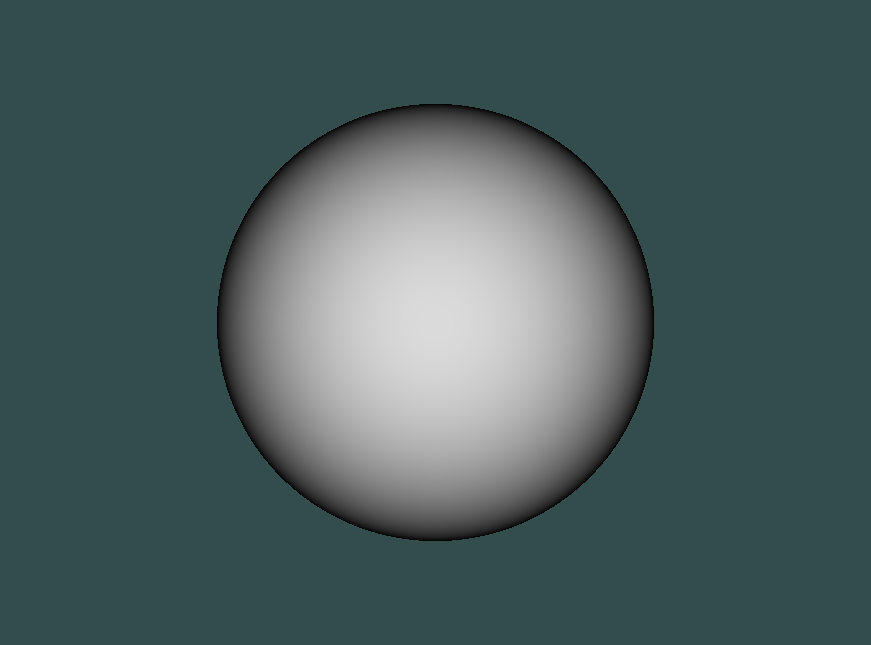
\includegraphics[width=1.0\textwidth]{render-regular.png}
    \end{minipage}
    \begin{minipage}{.2\textwidth}
      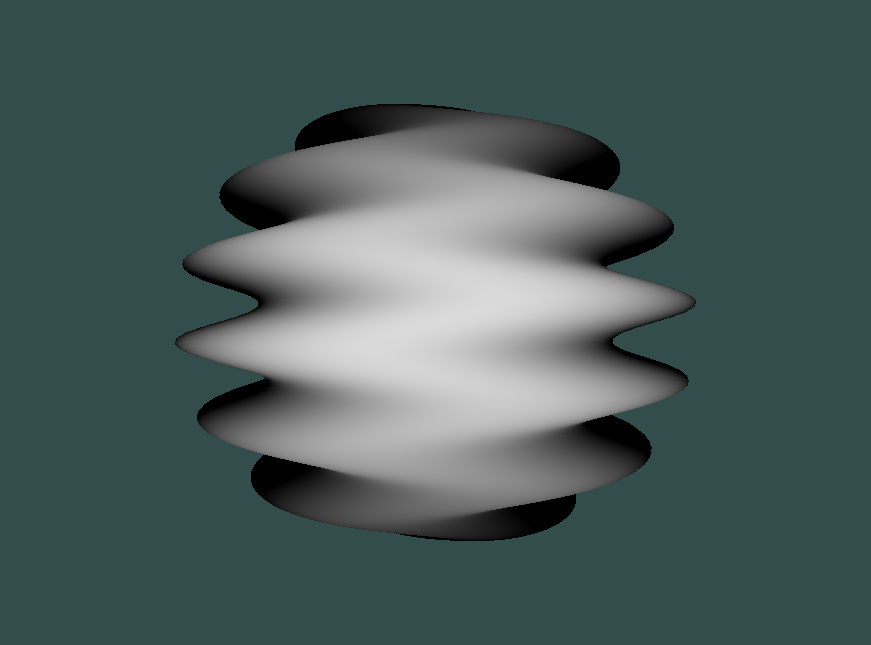
\includegraphics[width=1.0\textwidth]{render-warped.png}
    \end{minipage}
  \end{center}
  \caption{Left: rendering of a sphere using \autoref{lst:vertex}. Right: the same with \autoref{lst:warp} added.}
  \label{fig:regular}
\end{figure}

Using this technique, a wide variety of shaders can be combined, with a minimal amount of awareness of other shaders being necessary. Shortcomings of this technique are elaborated in \autoref{section:6}.

\section{Shader Integration with CLOS}\label{section:4}
Usually the shaders do not act on their own. They need corresponding CPU-side code in order to provide the inputs and parameters for the pipeline to execute properly. Thus our system couples the definition of relevant shader code and CPU code together in a single class. Combination of features is then automatically provided through the inheritance of classes. \\

We implement a new metaclass that includes a slot for a set of shader fragments, each grouped according to their pipeline stage. Shader fragments can then be attached to an instance of this metaclass to form the direct shader fragments. When the class hierarchy is finalised, shader fragments from all transitive superclasses are gathered in order of class precedence to form the list of effective shader fragments. This list is then combined into a full shader for each stage using the technique from \autoref{section:3}. \\

Accompanied by this metaclass is a set of generic functions that allow specifying the loading and drawing logic of a class. These functions encompass the CPU-side code required to run the shaders properly. Using the standard method combination, the behaviour can be passed down and combined alongside the shader code. An example of such a behaviour can be seen in \autoref{lst:colored-entity}.\\

\begin{listing}[h]
\begin{minted}[fontsize=\small]{common-lisp}
(defclass colored-entity ()
  ((color :initform (vec 0 0 1 1) :reader color))
  (:metaclass shader-class))

(defmethod paint :before ((obj colored-entity))
  (let ((shader (shader-program obj)))
    (setf (uniform shader "objectcolor") (color obj))))

(define-class-shader (colored-entity :fragment-shader)
  "uniform vec4 objectcolor;
out vec4 color;

void main(){
  color *= objectcolor;
}")
\end{minted}
\caption{A \code{colored-entity} class that encompasses object colouring functionality.}
\label{lst:colored-entity}
\end{listing}

This \code{colored-entity} class can now be used as a superclass in order to inherit the full behaviour. In effect this approach allows us to encapsulate a variety of small behaviours in the form of mixins, which can then be combined to form a full implementation of an object to be drawn. For instance, we could imagine an entity to emit geometry for a sphere, an entity to apply a wave deformation, an entity to texture the geometry, an entity to apply shading, and so forth.

\section{Applications}\label{section:5}
We currently use this technique for two primary applications: the encapsulation of common display functionality into mixins, and the implementation of effects passes. The former allows us to separate various concerns such as the read-out of texture data, the transformation of vertex data, and the fragment rendering behaviour into small, self-contained classes, that can then be combined by the user to produce the result they desire. \\

The latter allows us to write arbitrary rendering effects as self-contained render pass objects. To elaborate on this application, imagine a visual effect that requires you to manipulate some, but not all of the aspects of how an object is rendered. A simple example for such an effect is the ``god rays'' that you can see in \autoref{fig:godrays}. \\

In order to achieve this effect, all opaque objects in the scene are rendered once normally, and once in black. Then the black pass is blurred and added to the normal render. Neither the normal render pass nor the combination step require any insight from the pass into how the objects are drawn. However, for the black rendering pass, the way the objects are drawn has to be modified in such a way that all fragments are output as black, but everything else, such as vertex transformations, must remain the same. \\

With shader combination we can achieve this quite easily: we write a fragment shader that simply outputs the colour black, and then combine this shader with whatever the objects' shaders are. In this way we are virtually inserting a superclass for each object in the scene depending on which render pass is currently active. Render passes themselves are implemented with the same class shader combination as regular objects, so they too can profit from encapsulating and sharing shader functionality.

\begin{figure}[h]
  \begin{center}
    \begin{minipage}{.2\textwidth}
      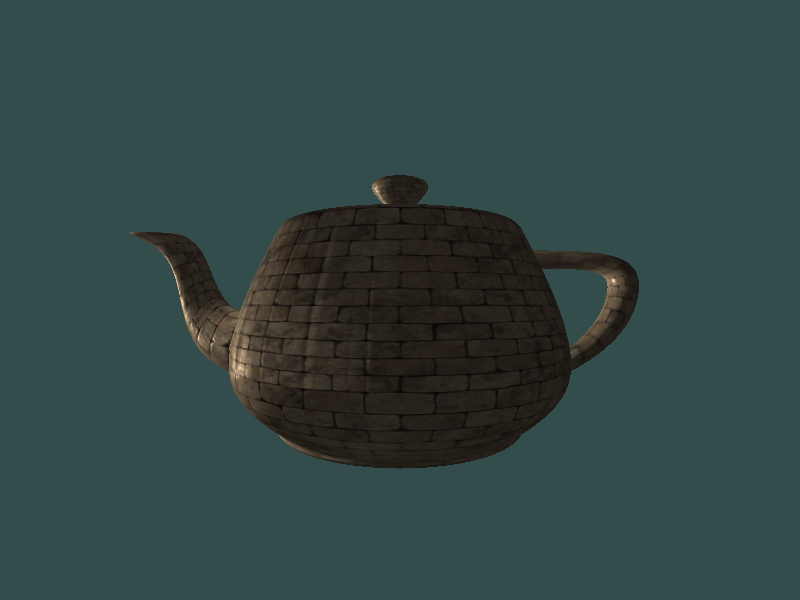
\includegraphics[width=1.0\textwidth]{pass-render.png}
    \end{minipage}
    \begin{minipage}{.2\textwidth}
      
\includegraphics[width=1.0\textwidth]{pass-black.png}
    \end{minipage}
    \vskip0.1cm
    \begin{minipage}{.4055\textwidth}
      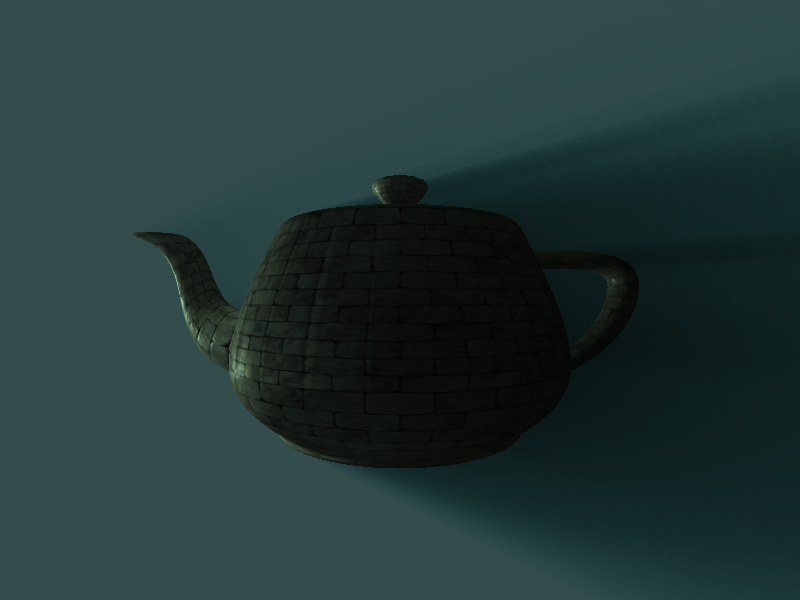
\includegraphics[width=1.0\textwidth]{pass-combined.png}
    \end{minipage}
  \end{center}
  \caption{Left: phong rendered teapot. Right: black rendered teapot. Bottom: combined god-rays effect.}
  \label{fig:godrays}
\end{figure}

\section{Conclusion}\label{section:6}
Source code analysis allows us to easily re-use shader code written independently of our Lisp program while retaining the ability to merge the effects of multiple shaders together. Integrating this analysis into the object system combines the GPU and CPU logic in a single class, allowing the inheritance and re-use of both. \\

While the merging works automatically for a large class of shaders, certain ambiguities cannot be automatically rectified and require user input. For instance, unless the names of \code{in} or \code{out} declarations match, or their location is explicitly specified, the static analysis cannot determine whether they denote the same thing. The shader effects that write to the same \code{out} variable must also be adapted to re-use the existing value in order for the effects to combine. For instance, a colour should be combined by multiplying with the previous value, rather than directly setting the new one. Typically multiplying the colour will yield the desired combination effect, whereas setting it would simply discard the colour computed by other mixins. Finally, if the declarations differ in qualifiers such as type or allocation, the merger cannot automatically determine how to resolve this conflict, even if the authors of the shaders meant it to denote the same conceptual variable.

\section{Further Work}\label{section:7}
The current merging strategy employed is rather simplistic. For instance, no attempt at recognising identical function definitions is made. The system could also be extended with a variety of static analysis algorithms to optimise the code ahead of time, or to provide errors and warnings about potential user mistakes. \\

While allowing the use of native GLSL code is handy, providing the user with a system to write shaders in Lisp syntax would improve the system quite a bit. To facilitate this change, the Varjo\cite{varjo} compiler could be integrated. A further development from there could be integration with an IDE to provide the user with automated help information about not just Lisp, but also shader functions.

\section{Acknowledgements}\label{section:8}
I would like to thank Robert Strandh and Philipp Marek for feedback on the paper.

\section{Implementation}\label{section:9}
An implementation of the proposed system can be found at \\\href{https://github.com/Shirakumo/trial/blob/e37e0dc73085c401e43da58d5098a9cf02167f8f/shader-entity.lisp}{https://github.com/Shirakumo/trial/blob/\\e37e0dc73085c401e43da58d5098a9cf02167f8f/shader-entity.lisp} \\ for the CLOS part, and at \url{https://github.com/Shirakumo/glsl-toolkit} for the merger part. \\

A more in-depth discussion of the system can be found at \\\url{https://reader.tymoon.eu/article/362}.

\bibliography{paper}
\end{document}

%%% Local Variables:
%%% mode: latex
%%% TeX-command-extra-options: "-shell-escape"
%%% TeX-master: t
%%% TeX-engine: luatex
%%% End:
